\documentclass{article}
\usepackage{amsmath, amssymb}
\usepackage[font=small,labelfont=bf]{caption} % Required for specifying captions to tables and figures
\usepackage[a4paper, total={6in, 8in}]{geometry}
\usepackage{listings}
\usepackage{multicol}
\usepackage[utf8]{inputenc}
\usepackage{tcolorbox}
\usepackage[dvipsnames]{xcolor}


% new tcolorbox environment
% #1: tcolorbox options
% #2: color
% #3: box title
\newtcolorbox{ejemplo}[1][]
{
  colframe = blue!25,
  colback  = blue!10,
  coltitle = blue!20!black,  
  title    = {\textbf{Ejemplo de uso}},
  #1,
}

\newcommand{\breakcol}{\vfill\null \columnbreak}
\newcommand{\comma}{,\;}

\title{EDA FINAL}
\author{Nicolás Margenat}
\date{2022 1Q}

\begin{document}

\maketitle

\tableofcontents

\newpage
\section{Complejidades}
\begin{multicols}{2}

\textbf{LEVENSHTEIN}:
\begin{itemize}
    \item \emph{Temporal}: $O(n*m)$ 
    \item \emph{Espacial}: $O(n*m)$ 
\end{itemize}
donde $n$ y $m$ son las longitdes del $str1$ y $str2$ respectivamente.

\textbf{KMP}:
\begin{itemize}
    \item \emph{Temporal}: $O(m)$ 
    \item \emph{Espacial}: $O(m)$ 
\end{itemize}
donde $m$ es la longitud del query.

\textbf{BINARY SEARCH}:
\begin{itemize}
    \item \emph{Temporal}: $O(log_2(N))$ (recursiva e iterativa)
    \item \emph{Espacial}: $O(log_2(N))$ (recursiva) y $O(1)$ (iterativa)
\end{itemize}

\textbf{QUICKSORT}:
\begin{itemize}
    \item \emph{Temporal}: $O(N^2)$ 
    \item \emph{Espacial}: $O(N)$ 
\end{itemize}

\textbf{MERGESORT}:
\begin{itemize}
    \item \emph{Temporal}: $O(N*log_2(N))$ 
    \item \emph{Espacial}: $O(N)$ 
\end{itemize}

\breakcol
\textbf{BFS}:
\begin{itemize}
    \item \emph{Temporal}: $O(V + E)$ 
    \item \emph{Espacial}: $O(V)$ (usa Cola)
\end{itemize}

\textbf{DFS}:
\begin{itemize}
    \item \emph{Temporal}: $O(V + E)$ 
    \item \emph{Espacial}: $O(V)$ (usa Stack)
\end{itemize}

\textbf{AVL}:
\begin{itemize}
    \item \emph{Temporal}: $O(log_2(N))$ 
    \\(inserción, borrado, búsqueda)
    \item \emph{Espacial}: $O(N)$ 
\end{itemize}

\textbf{BTree}:
\begin{itemize}
    \item \emph{Temporal}: $O(N)$ 
    \\(inserción, borrado, búsqueda)
\end{itemize}

\textbf{RED-BLACK TREE}:
\begin{itemize}
    \item \emph{Temporal}: $O(log_2(N))$ 
    \\(inserción, borrado, búsqueda)
    \item \emph{Espacial}: $O(N)$ 
\end{itemize}

\textbf{BST}:
\begin{itemize}
    \item \emph{Temporal}: $O(N)$ 
    \\(inserción, borrado, búsqueda)
    \item \emph{Espacial}: $O(N)$ 
\end{itemize}

\end{multicols}

%-----------------------------------------------------------------------
\newpage
\section{Lucene}
Lucene usa un \emph{archivo invertido}: conjunto de términos que indican a qué documento pertenece.
\begin{equation*}
    \text{término $\rightarrow$ documento} 
\end{equation*}

\subsection{Definiciones}
\subsubsection*{Definición 1. Documento Lucene}
Secuencia de \emph{campos (fields)}. Cuando se ingresa un documento en Lucene automáticamente se le asocia un ID (docid).

\subsubsection*{Definición 2. Campo/Field}
Par nombre-secuencia de $1+$ términos.
\\Un field puede ser:
\begin{enumerate}
    \item Sólo almacenable (se guarda literal y no se procesa) $\Rightarrow$ está fuera del archivo invertido, por lo que \textbf{no} participa de las búsquedas
    \item Sólo indexable $\Rightarrow$ participa de las búsquedas
    \item Indexable y almacenable $\Rightarrow$ se guarda literal y se procesa para que participe de las búsquedas
\end{enumerate}
El \emph{field predefinido} es \textbf{TextField}: maneja tipos de datos de texto, se indexa y se tokeniza.

\subsubsection*{Definición 3. Término/Term}
Un término Lucene es una secuencia de bytes (int, string, etc) asociada a cierto campo.
Es importante notar que \emph{dos secuencias de bytes con igual contenido pero asociadas a 2 campos diferentes se consideran diferentes}.
\\\underline{Ejemplo}: Dato (título materia) $\neq$ Dato (apellido)

\subsection{Aplicaciones}
Necesitamos realizar dos aplicaciones independientes con Lucene: \textbf{IndexBuilder} y \textbf{Searcher}.
\subsubsection{IndexBuilder}
Aplicación que se encarga de generar el índice a partir de un conjunto de documentos Lucene y lo deja almacenado en un directorio que le digamos.
\begin{center}
    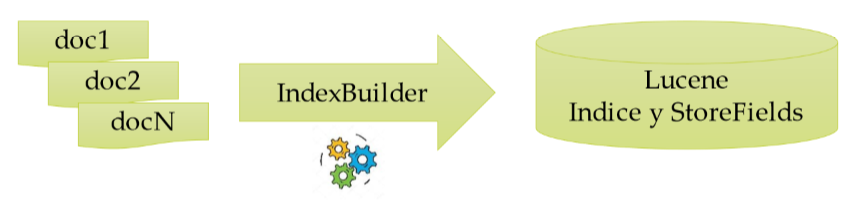
\includegraphics[width=.70\textwidth]{Images/IndexBuilder.png}
\end{center}
\underline{Observación}: Es nuestra responsabilidad mantener el índice actualizado, es decir: re-ejecutar si agregamos o modificamos documentos.

\subsubsection{Searcher}
Aplicación que se encarga de aceptar consultas y utiliza el índice construido para retornar los docids que "matchearon" la consulta rankeados en cierto orden.
\begin{center}
    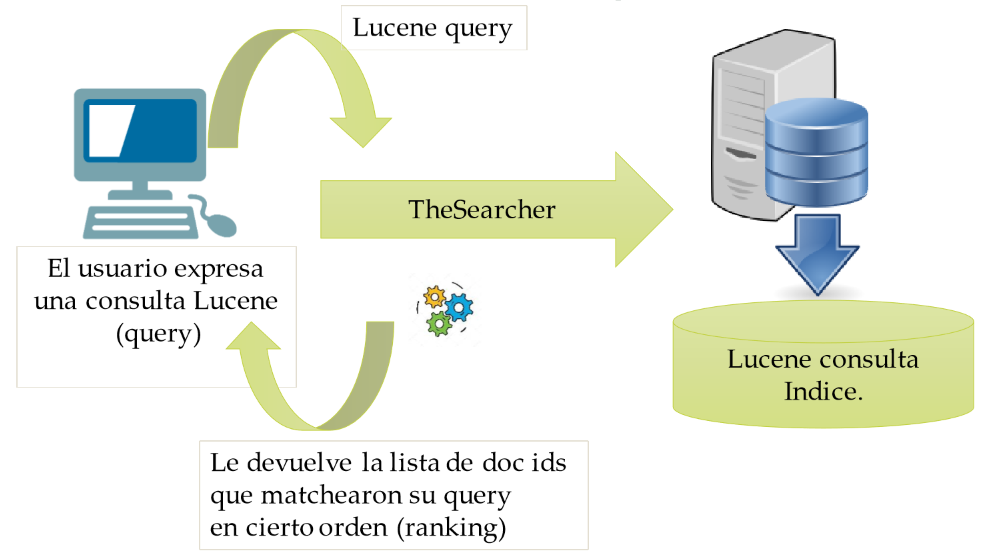
\includegraphics[width=.60\textwidth]{Images/Searcher.png}
    \captionof{figure}{Proceso de Búsqueda}
\end{center}
\begin{center}
    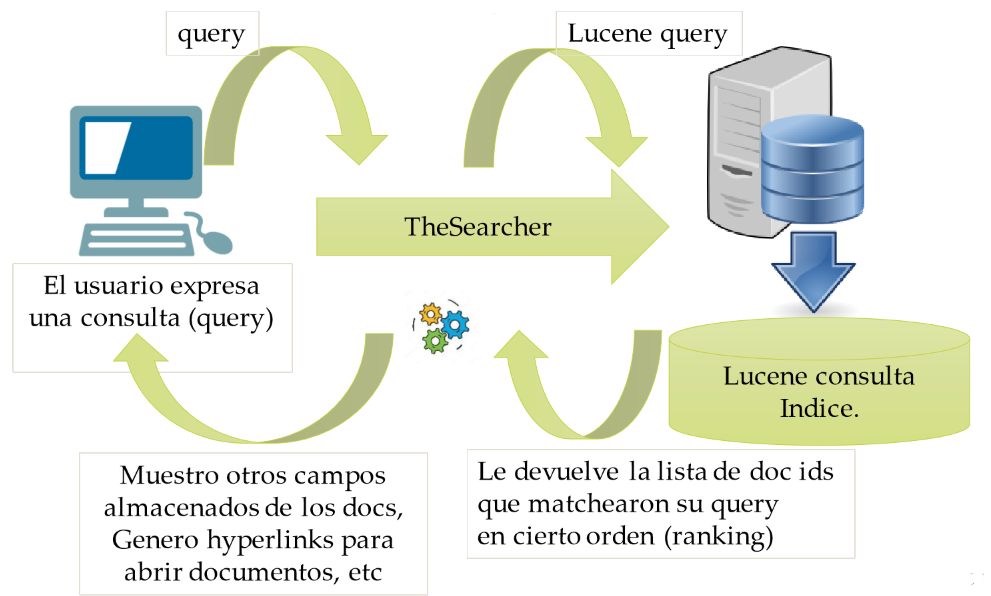
\includegraphics[width=.60\textwidth]{Images/SearcherMejorado.png}
    \captionof{figure}{Proceso de Búsqueda Mejorado}
\end{center}

\subsection{Queries}
\subsubsection{TermQuery}
Busca \textbf{un} sólo término.

\subsubsection{PrefixQuery}
Busca por prefijo.

\subsubsection{TermRangeQuery}
Busca si el término se encuentra en el intervalo especificado.
\begin{center}
    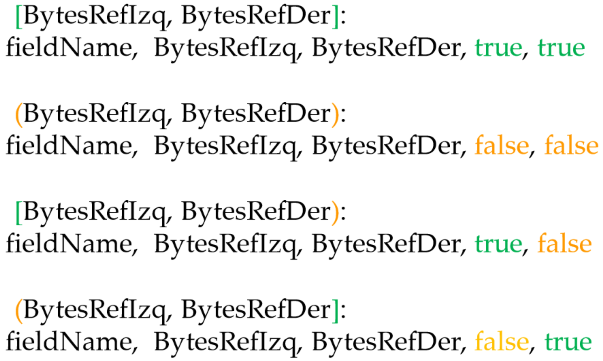
\includegraphics[width=.40\textwidth]{Images/TermRangeQuery.png}
\end{center}

\subsubsection{PhraseQuery}
Busca secuencia.
\begin{ejemplo}
\begin{lstlisting}
Query query = new PhraseQuery(fieldName, word1, word2
                                , ..., wordN);
\end{lstlisting}
\end{ejemplo}

\subsubsection{WildcardQuery}
Busca por matching de $*$ o bien $?$.
\begin{ejemplo}
\begin{lstlisting}
Query query = new WildcardQuery(myTerm);
\end{lstlisting}
Algunos ejemplos:
\begin{lstlisting}
queryStr = "g*e";   // g(0 <= letras)e
queryStr = "g?e";   // g(1 >= letras)e
queryStr = "*";     // (0 <= letras)
\end{lstlisting}
\end{ejemplo}

\subsubsection{FuzzyQuery}
Usa Damerau-Levenshtein con MaxEdit 2.

\subsubsection{BooleanQuery}
Es como una expresión de Lógica Proposicional.
\begin{ejemplo}
\underline{Ejemplo 1}:
\begin{lstlisting}
String queryStr = "game AND store";
QueryParser queryParser = new QueryParser("content", 
                                            new StandardAnalyzer());
\end{lstlisting}

\underline{Ejemplo 2}:
\begin{lstlisting}
String queryStr = "game OR store";
QueryParser queryParser = new QueryParser("content", 
                                            new StandardAnalyzer());
\end{lstlisting}
\end{ejemplo}

\subsection{Ranking}
Dada una colección de $N$ documentos $D = \{ Doc_1 \comma Doc_2 \comma  ... \comma Doc_n \}$ y una $query = term$, para aquellos documentos que matchean la consulta:
\begin{equation*}
    Score(Doc_i \comma query) = FormulaLocal(Doc_i \comma term) * FormulaGlobal(D \comma term)
\end{equation*}
donde
\begin{itemize}
    \item \underline{Fórmula Local}: Calcula qué tan relevante es un query respecto al documento a rankear.
    \begin{equation*}
        FormulaLocal(Doc_i \comma query) = \sqrt{\frac{\#freq(term \, in \, Doc_i)}{\#term \, existentes \, en \, Doc_i}}
    \end{equation*}
    \item  \underline{Fórmula Global}: Calcula qué tan relevante es esa query en el conjunto de documentos. 
    \begin{equation*}
        FormulaGlobal(DOC \comma query) = 1 + log_e\left(\frac{1 + \#docs \, en \, la \, coleccion}{1 + \#docs \, que \, contienen \, term}\right)
    \end{equation*}
\end{itemize}

\subsubsection*{Ranking Multi-Término}
Si un query consta de varios términos entonces el puntaje se calcula:
\begin{equation*}
    Score(Doc_i \comma query) = \sum_{\substack{\text{term in query}\\ \text{y no tiene NOT}}} FormulaLocal(Doc_i \comma term) * FormulaGlobal(D \comma term)
\end{equation*}
es decir, se hace la sumatoria de los calculos parciales de cada término del query sii no está modificado por NOT.

%-----------------------------------------------------------------------
\newpage
\section{Teorema Maestro}
Si una fórmula recurrente puede expresarse genéricamente así:
\begin{equation*}
    T(N) = \underbrace{a*T(\frac{N}{b})}_{\substack{\text{Invocación recursiva que}\\ \text{divide en subproblemas}}} + \underbrace{c * N^d}_{\substack{\text{Combinación de}\\ \text{soluciones parciales}}}
\end{equation*}
Entonces la complejidad $O$ grande está dada por los siguientes 3 casos:
\begin{enumerate}
    \item Si $a < b^d \Rightarrow O(N^d)$
    \item Si $a = b^d \Rightarrow O(N^d * log(N))$
    \item Si $a > b^d \Rightarrow O(N^{log_b(a)})$
\end{enumerate}
donde 
\begin{itemize}
    \item $N$ es el tamaño del input
    \item $a \in \mathbb{N}_{\geq 1}$ invocaciones recursivas por paso
    \item $b \in \mathbb{N}_{> 1}$ mide tasa en que se reduce el tamaño del input
    \item $c \in \mathbb{R}_{>0}$
    \item $d \in \mathbb{R}_{\geq 0}$
\end{itemize}

%-----------------------------------------------------------------------
\newpage
\section{Algoritmos}
\subsection{Red-Black Trees}
\subsubsection*{Reglas}
\begin{enumerate}
    \item Cada nodo es \textbf{\textcolor{red}{ROJO}} ó \textbf{NEGRO}
    \item La raíz \underline{siempre} es \textbf{NEGRA}
    \item Las hojas \underline{siempre} son \textbf{NEGRAS}
    \item Las nuevas inserciones son \textbf{\textcolor{red}{ROJAS}}
    \item Cada camino de la raíz a las hojas tiene la \underline{misma} cantidad de nodos \textbf{NEGROS}
    \item \underline{No} puede haber nodos \textbf{\textcolor{red}{ROJOS}} consecutivos
\end{enumerate}

\subsubsection*{Rebalanceo}
Tenemos dos casos:
\begin{enumerate}
    \item "\textbf{BLACK} Aunt Rotate (BAR)" 
    \begin{center}
        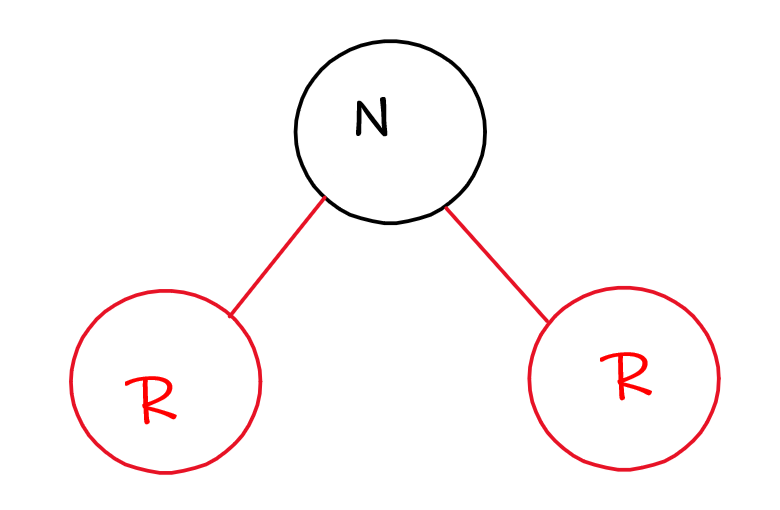
\includegraphics[width=.25\textwidth]{Images/Rotate.png}
        \captionof*{figure}{Después de Rotar}
    \end{center}
    \item "\textbf{\textcolor{red}{RED}} Aunt Colorflip (RAC)"
    \begin{center}
        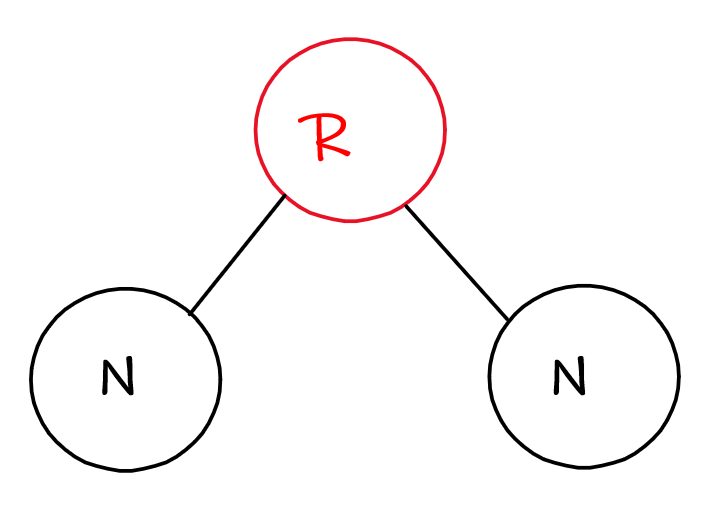
\includegraphics[width=.25\textwidth]{Images/Colorflip.png}
        \captionof*{figure}{Después del Colorflip}
    \end{center}
\end{enumerate}

\subsection{Soundex}
\begin{enumerate}
    \item Utiliza una cartilla para codificar las letras:
    \begin{center}
        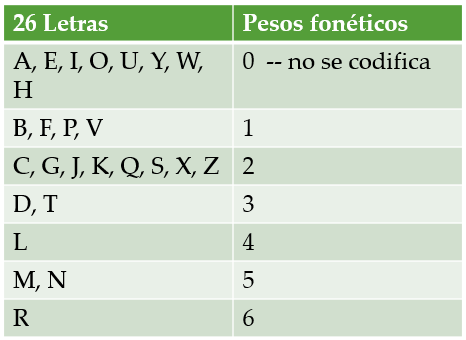
\includegraphics[width=.40\textwidth]{Images/SoundexTabla.png}
    \end{center}
    \item Siempre devuelve un código OUT de 4 caracteres, formado por: primero una letra y 3 dígitos (pesos fonéticos). Si hace falta se completa con 0s.
    \item \underline{Algoritmo en C}:
    \begin{center}
        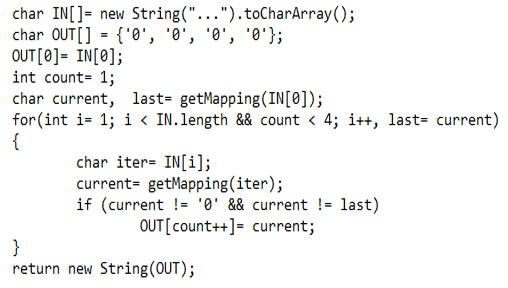
\includegraphics[width=.60\textwidth]{Images/SoundexAlgoritmo.png}
    \end{center}
    \item \underline{Algoritmo papel}:
    \begin{center}
        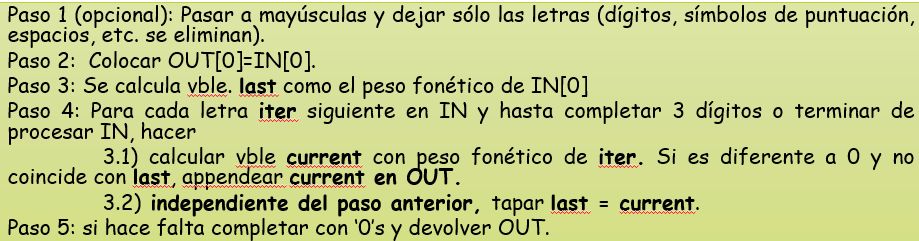
\includegraphics[width=.60\textwidth]{Images/SoundexAlgoritmoPapel.png}
    \end{center}
    \item \textbf{Similitud para Soundex}: Es la longitud de caracteres coincidentes entre los encodings respecto a la longitud del encoding. Por lo tanto los valores posibles son: $0, 0.25, 0.5, 0.75, 1$.
\end{enumerate}
    
\subsection{Levenshtein Distance}
\underline{Definición}: Es un algoritmo que calcula la mínima cantidad de operaciones necesarias para transformar un string a otro. Las operaciones validas son: \emph{insertar, borrar o sustituir un caracter}.

\begin{enumerate}
    \item Es una \textbf{métrica de distancia}, por lo que cumple con las siguientes propiedades:
        \subitem \underline{Simetria}: Lev(str1, str2) = Lev(str2, str1)
        \subitem \underline{Desigualdad}: Lev(str1, str2) + Lev(str2, str3) $\geq$ Lev(str1, str3)
    \item Se lo implementa con Programación Dinámica (= tecnica que consiste en reusar valores previamente calculados para no tener que recalcularlos repetidamente)
    \item Se utiliza una tabla para poner en practica la Programación Dinámica:
    \begin{center}
        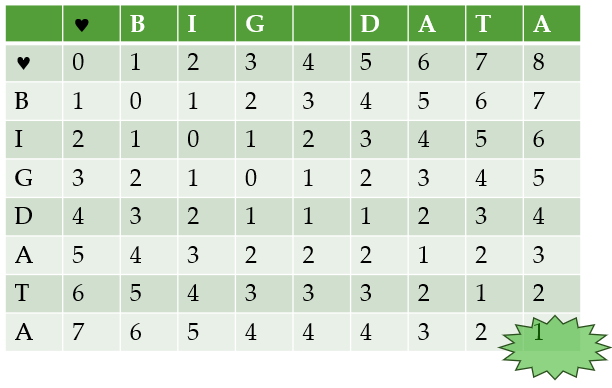
\includegraphics[width=.60\textwidth]{Images/LevenshteinTable.png}
    \end{center}
    donde cada celda representa la distancia entre el substring de arriba y el de la izquierda.
    \item Para calcular una celda, se le suma uno a la de la izquierda, uno al de arriba y para la diagonal (de arriba a la izquierda) hay dos opciones: se le suma 0 si las letras coinciden, y 1 si no coinciden.
    \item Se puede normalizar el resultado de la siguiente manera:
    \begin{equation*}
        LevNormalized(str1, str2) = 1 - \frac{Lev(str1, str2)}{max(str1.length(), str2.length())}
    \end{equation*}
\end{enumerate}

\subsection{Q-Grams}
\underline{Definición}: Es un algoritmo que consiste en generar los pedazos que componen un string. La distancia entre 2 strings estará dada por la cantidad de componentes que tengan en común.
\begin{enumerate}
    \item \underline{Canónica}: 
    \subitem Se toman hasta ventanitas de tamaño 3.
    \subitem Para que todas las letras participen lo mismo se le ponen $Q - 1$ metacaracteres en los extremos (donde $Q$ es la cantidad de letras).
    \item La forma de normalizarlo es la siguiente:
    \begin{equation*}
        QGram(str1, str2) = \frac{\#TG(str1) + \#TG(str2) - \#TGNoShared(str1, str2)}{\#TG(str1) + \#TG(str2)}
    \end{equation*}
    entonces 1 es maxima similitud y 0 es nula.
    \item \emph{Ejemplo}:
    \begin{center}
        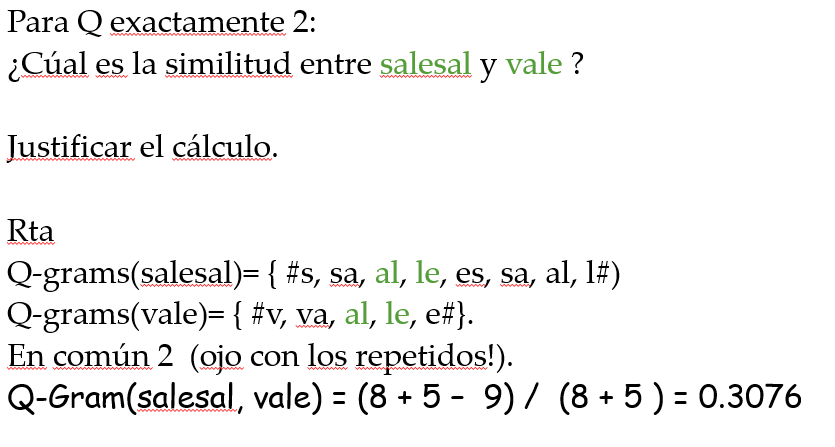
\includegraphics[width=.50\textwidth]{Images/QGramEj.png}
    \end{center}
\end{enumerate}

\subsection{KMP}
\begin{enumerate}
    \item No vuelve a chequear un carácter que ya sabe que matcheó.
    \item Utiliza la tabla de "Next" que tiene en cada posición $i$ la longitud del \emph{borde propio} más grande para el substring query desde 0 hasta $i$.
    \item Para calcular la tabla "Next" se utiliza el siguiente algoritmo:
    \begin{center}
        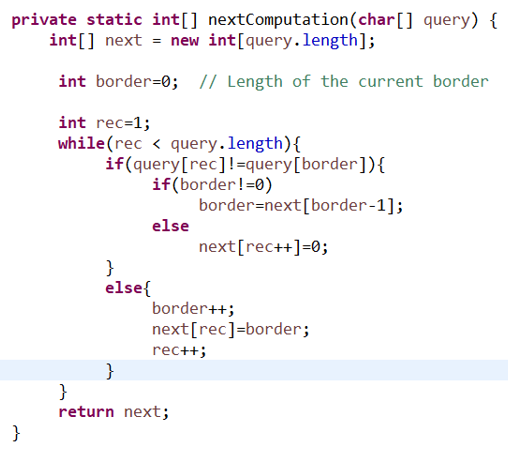
\includegraphics[width=.50\textwidth]{Images/AlgNext.png}
    \end{center}
    \item \textbf{Algoritmo KMP}
        \begin{center}
        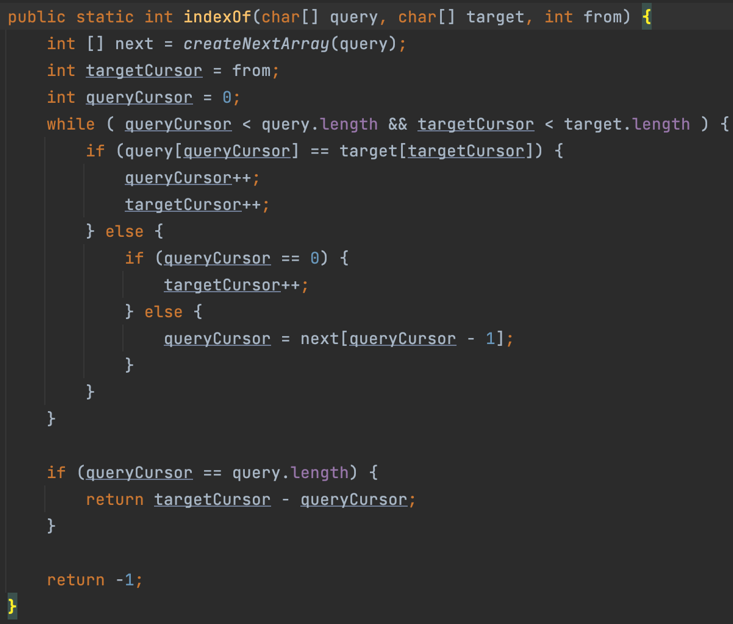
\includegraphics[width=.50\textwidth]{Images/KMPAlgoritmo.png}
    \end{center}
\end{enumerate}
\textbf{Complejidades}:
\begin{itemize}
    \item Next:
    \subitem \underline{Espacial}: $O(m)$
    \subitem \underline{Temporal}: $O(m)$
    donde $m$ es la longitud del query.
\end{itemize}

%-----------------------------------------------------------------------
\newpage
\section{Heurísticas}
\subsection{Fuerza Bruta/Búsqueda Exhaustiva (con Stack o Queue)}
\begin{tcolorbox}[title=Definición]
Técnica que busca todas las posibles soluciones explorando el espacio de soluciones de forma implícita.
\end{tcolorbox}
Se usa si un problema tiene muchas soluciones y las quiero todas.

\subsubsection*{Idea}
\begin{enumerate}
    \item Si el nodo no puede expandirse más $\Rightarrow$ retornar/imprimir resultado
    \item Sino por cada posibilidad para ese nodo expandir en un próximo nivel. El nodo puede:
        \subitem Resolver caso pendiente
        \subitem Explorar nuevos pendientes
        \subitem Deshacer/Quitar pendiente generado
\end{enumerate}

\subsection{Programación Dinámica}
\begin{tcolorbox}[title=Definición]
Técnica que permite almacenar valores que se calcularon previamente en soluciones anteriores para reusarlos, en vez de calcularlos repetidamente.
\end{tcolorbox}
\underline{Ejemplo}: Levenshtein, Dijkstra, Ackerman, Fibonacci.

\subsection{Backtracking}
\begin{tcolorbox}[title=Definición]
No expande innecesariamente nodos que ya sabe (gracias a las restricciones) que \underline{no} conducen a la solución.
\end{tcolorbox}
\textbf{¿Cómo evita expandir más de un nodo?}
Un nodo intermedio ya lleva acumulado valores. 
En el mejor de los escenarios completará con números bajos, es decir “1” en lo que falta.
\begin{equation*}
    \text{Si }\sum{}{} \left(\text{valores actuales}\right) + \text{ valores faltantes} * 1 > \text{umbral} \Rightarrow \text{imposible seguir}
\end{equation*}
\underline{Ejemplo}: N-Queens.

\subsubsection*{Backtracking + Programación Dinámica}
Con programación dinámica podemos agregar la suma actual como parámetro y así evitar calcular muchas veces la suma.

\subsection{Divide \& Conquer}
\begin{tcolorbox}[title=Definición]
Técnica que descompone un problema de tamaño $N$ en problemas más pequeños que tengan solución. Finalmente, se debe proponer cómo construir la solución final a partir de las soluciones de los problemas menores.
\end{tcolorbox}
\underline{Ejemplo}: Mergesort, Quicksort, Búsqueda en BST.

\subsection{Algoritmos Greedy/Ávidos}
\begin{tcolorbox}[title=Definición]
Técnica que busca en cada etapa un óptimo local con el objetivo de llegar al óptimo global.
\end{tcolorbox}
\underline{Ejemplo}: Algoritmo de Kruskal.


\end{document}
